% Submission to Scientific Programming: adapted from paper in ICCS2006,
% "Workflow systems in e-Science" workshop

% Changes from WSES workshop paper:
% * Reworked intro
% * More on security and (GSI)-SSH
% * Added section on running on Condor/SGE
% * Added two figures

\documentclass[a4paper]{article}

\usepackage{graphicx}
\usepackage{setspace}
\usepackage{caption}
\usepackage{alltt}
\usepackage[left=40mm, right=40mm, top=40mm, bottom=40mm]{geometry}

% Make figures come out as "Fig. 1" instead of "Figure 1"
\renewcommand{\figurename}{Fig.}

% I tried to create a bibtex style file for Scientific Programming but didn't get it quite right...
%\bibliographystyle{sciprog}
\bibliographystyle{plain}

\begin{document}
\doublespacing

\begin{center}
{\Large Styx Grid Services: Lightweight, easy-to-use middleware for scientific workflows}

\bigskip
\bigskip

{\large J.D. Blower$^{1}$, A.B. Harrison$^{2}$ and K. Haines$^{1}$}

\bigskip

{\small 1. \textit{Reading e-Science Centre, Environmental Systems Science Centre, \\
University of Reading, Reading RG6 6AL, UK} \\
Email: \{jdb, kh\}@mail.nerc-essc.ac.uk\\
Tel: +44 118 378 8741 \\
\medskip
2. \textit{School of Computer Science, Cardiff University, Cardiff CF24 3AA, UK}\\
Email: a.b.harrison@cs.cardiff.ac.uk\\
Tel: TODO}

\bigskip
\bigskip

Keywords: streaming, third-party transfers, WS-RF, Condor, Globus

\end{center}

\newpage

\begin{abstract}
The service-oriented approach to performing distributed scientific research is potentially very powerful but is not yet widely used in many scientific fields.  This is partly due to the technical difficulties involved in creating services and composing them into workflows.  We present the Styx Grid Service, a simple system that wraps command-line programs and allows them to be run over the Internet exactly as if they were local programs.  Styx Grid Services are very easy to create and use and can be composed into powerful workflows with simple shell scripts or more sophisticated graphical tools.  Data can be streamed directly from service to service and progress can be monitored asynchronously using a mechanism that places very few demands on firewalls.  Styx Grid Services can be used as an easy-to-use, uniform interface to Condor and Globus resources, permitting the creation of workflows that span various Grid resources.  We shall show how Styx Grid Services can interoperate with Web Services and WS-Resources.
\end{abstract}

\section{Introduction}\label{sec:intro}
The use of service-oriented architectures (SOAs) in scientific computing is increasing.  The principal advantage of the SOA approach is that scientists can access resources such as databases, high-end computing resources, laboratory equipment and sensor networks over the Internet without knowledge of the underlying infrastructure.  Several independent services can be combined in a distributed application or \textit{workflow\/} to solve a particular problem.  For example, a scientist might wish to construct a workflow in which several pieces of data are extracted from databases in different locations, analyzed using a distributed computing resource, then finally visualized on his or her local machine.

At present, however, there are very few examples of scientific communities that work routinely in this way.  The reasons for this include:

\begin{itemize}
\item The creation of such services is beyond the technical expertise of most scientists and so very few services exist for scientists to use.
\item The process of constructing workflows from these services is also technically challenging.
\item Many service providers employ complex security frameworks that are hard to use.
\end{itemize}

Web Services, although designed primarily for business-to-business interaction, are seeing increasing use in distributed scientific computing.  They provide significant advantages for creating loosely-coupled, interoperable services: they are accessed through XML messaging and are thus inherently cross-platform, they are self-describing (through Web Service Definition Language -- WSDL -- documents) and are a widely-accepted standard for distributed computing.  However, Web Services have some important limitations in the context of scientific workflows. In particular, it is impractical to encode anything but a small amount of data in XML due to the processing time required and the inflating effect of doing so.  Furthermore, scientific services are often long-running and so it is highly desirable to be able to monitor the progress and status of the service as it runs using asynchronous notifications.  Solutions such as the Web Services Resource Framework (WSRF~\cite{WSRF}) employ notification mechanisms that require the client to run a server process.  This requirement means that clients that are behind stringent firewalls or Network Address Translation (NAT) systems will not receive these notifications.

We describe a service type that addresses the above issues: the \textit{Styx Grid Service} or SGS.  A Styx Grid Service is a service that wraps a command-line (i.e.\ non-graphical) program and allows it to be run remotely.  The key features of the SGS system are:

\begin{itemize}
\item Scientists can write a program in their language of choice, then deploy it as a Styx Grid Service with minimal effort.
\item Clients can run remotely-deployed SGSs exactly as if they were local programs.
\item Simple workflows can be created using shell scripts.  Clients can create more complex workflows through more sophisticated tools.
\item SGSs can be used as a uniform front end to Condor pools, Globus resources and other distributed computing facilities, simplifying their use.
\item Data can be streamed directly between service instances in the most compact binary form, meaning that the workflow enactor does not have to process these intermediate data.
\item SGSs can interoperate with Web Services through suitable adapters.
\end{itemize}

\section{Styx Grid Services: overview}\label{sec:sgsoverview}
Our main goal in developing the Styx Grid Services system was to create remote services that are used exactly as if they were local programs.  The basis of the system is the Styx protocol for distributed systems.  

\subsection{The Styx protocol}
Styx~\cite{Pike:1999} is a well-established protocol for building distributed systems: it is a key component of the Inferno \cite{Inferno} and Plan~9 \cite{Plan9} operating systems (in Plan~9, Styx is known as ``9P'': the current version of Styx is equivalent to 9P2000).  In Inferno and Plan~9, applications communicate with all resources using Styx, without knowing whether the resources are local or remote.  Styx is essentially a file-sharing protocol, similar in some ways to NFS.  However, in a Styx system the ``files'' are not always literal files on a hard disk.  They can represent a block of RAM or the interface to a program, database or physical device.  Styx can therefore be used as a uniform interface to access diverse resource types.  Whereas in Remote Procedure Call (RPC)-style Web Services the resources are accessed through a set of methods, Styx resources are accessed by reading from and writing to a hierarchy of files, which is known as a \textit{namespace\/}.

We developed a pure-Java implementation of the Styx protocol (JStyx~\cite{JStyx}) and used this as the basis for the Styx Grid Services software..

\subsection{The SGS namespace}\label{sec:sgsnamespace}
The namespace of a typical Styx Grid Service server is shown in Fig.~\ref{fig:sgsnamespace}.  A server can host several Styx Grid Services, which are each represented as a directory in the namespace.  A more detailed description of the purpose of the files in the namespace can be found on the project website~\cite{sgswebsite}.

% When a client executes a Styx Grid Service, it performs the following basic steps: (1) The client reads from the \texttt{clone} file to create a new instance of the service.  This instance appears as a new directory in the \texttt{instances} directory of the namespace.  (2) The client sets the parameters of the service instance by writing to the files in the \texttt{params} directory.  (3) The client uploads the necessary input files by writing them into the \texttt{inputs} directory.  (4) The client starts the service by writing the string \texttt{start} into the \texttt{ctl} (control) file.  (5) Progress and status notifications are obtained by reading from the files in the \texttt{serviceData} directory.  (6) The client downloads the resulting output files from the \texttt{outputs} directory.

Due to the filesystem-like structure of the namespace, every resource on an SGS server can be identified naturally and uniquely as a URL.  For example, the file that represents the standard output stream of instance \texttt{1} of the the \texttt{mySGS} service can be identified by \texttt{styx://<server>:<port>/mySGS/instances/1/outputs/stdout}.  This is very important in the context of workflows: these URLs are passed between services in a workflow as data pointers, to enable direct transfer of data between services (see Sect.~\ref{sec:datapassing}).

\subsection{Security}\label{sec:security}
The Styx protocol itself deliberately does not mandate any particular security mechanism.  The JStyx software permits the SGS server to run in two modes, each with a different security mechanism:

In \textit{daemon mode}, the SGS server runs as a persistent daemon (server process) as a generic user, exchanging Styx messages on a single network socket.  In this mode, users authenticate through a custom mechanism and the SGS server administrator must maintain a dedicated user database.  Traffic between the client and the server can optionally be encrypted using SSL (Secure Sockets Layer).

In \textit{tunnelled mode}, users log on to the SGS host through the Secure Shell (SSH), then execute an SGS server process that runs \textit{with the permissions of the user in question}.  This process exchanges Styx messages on its standard input and output streams and these messages are directed to and from the client over the network through the secure SSH tunnel.  There is no dedicated user database.  If Globus security is required, GSI-SSH can be used in place of SSH: in this case, users authenticate through X.509 proxy certificates~\cite{blower_ahm:2006}.

In either case, the SGS server only requires a single incoming port to be open through its firewall: a single server program handles all tasks such as file transfers, control messages and notifications.  Since clients interact with the server through persistent connections, clients require \textit{no} incoming ports to be open: furthermore the client can be behind a NAT router.  This is how we solve the problem of asynchronous notification that was discussed in section~\ref{sec:intro} above.  Hence SGS servers can be deployed easily and securely.


\section{Creating Styx Grid Services}\label{sec:wrapping}
Neither service providers nor end-users need to know anything about the technical details discussed in section~\ref{sec:sgsoverview} above.  The process of wrapping a command-line program as a Styx Grid Service is very simple.  Let us take the example of a simple visualization program called \texttt{makepic} that reads an input file and creates a visualization of the results as a PNG (Portable Network Graphics) file.  The names of the input and output files are specified on the command line, for example:

\begin{verbatim}
   makepic -i input.dat -o pic.png
\end{verbatim}

This program can be deployed on a server as a Styx Grid Service as follows.  The \texttt{makepic} program is installed on the SGS server.  The service provider creates a simple XML configuration file that describes the program completely in terms of its inputs, outputs and command-line arguments (see Fig.~\ref{fig:makepicconfig}).  The SGS server program parses this configuration file and sets up the SGS namespace (Fig.~\ref{fig:sgsnamespace}).  The \texttt{makepic} executable file itself cannot be accessed directly by clients.

\subsection{Executing SGSs just like local programs}

Once the \texttt{makepic} program is deployed as a Styx Grid Service, clients can run the service from remote locations, exactly as if the \texttt{makepic} program were deployed on their local machines.  They do this using the \texttt{SGSRun} program, which is a generic client program for running any SGS:

\begin{verbatim}
   SGSRun <hostname> <port> makepic -i input.dat -o pic.png
\end{verbatim}
where \texttt{<hostname>} and \texttt{<port>} are the host name (or IP address) and port of the SGS server respectively.  The \texttt{SGSRun} program connects to the SGS server and downloads the XML description of the \texttt{makepic} program  (Fig.~\ref{fig:makepicconfig}).  \texttt{SGSRun} uses this configuration information to parse the command line arguments that the user has provided.  It then knows that the local file \texttt{input.dat} is an input file and uploads it automatically from the user's machine to the SGS server before the service is started.  Having started the service, \texttt{SGSRun} knows that \texttt{makepic} will produce an output file called \texttt{pic.png}, which it downloads to the user's machine.  (For programs that use the standard streams -- \texttt{stdout}, \texttt{stderr} and \texttt{stdin} -- these are redirected to and from the console as appropriate.)

It is a very easy task to create a simple shell script (or batch file in Windows) called \texttt{makepic} that wraps the \texttt{SGSRun} program and contains the host name and port of the SGS server, so the user can simply run:

\begin{verbatim}
   makepic -i input.dat -o pic.png
\end{verbatim}
exactly as before.  The \texttt{makepic} script (which calls the remote Styx Grid Service) behaves identically to the original executable.


\section{Creating workflows with shell scripts}\label{sec:shellscripts}

Given that remote SGSs can be executed exactly like local programs, workflows can be created with simple shell scripts.  Workflows are simply high-level programs and so it is natural to use a scripting environment to create them.  This allows SGSs to be combined easily with local programs and permits the use of all the programming features that the scripting language provides.  Let us consider a simple workflow of two Styx Grid Services.  The first is a service called \texttt{calc\_mean} that takes a set of input files and calculates their mean (this service might, for example, calculate the mean of an ensemble of climate forecasts).  The second SGS is the \texttt{makepic} service from section~\ref{sec:wrapping} above, which is used to visualize the mean data.  The shell script (workflow) that would be used to take a set of input files, calculate their mean and plot the result would be:

\begin{verbatim}
   calc_mean input*.dat -o mean.dat
   makepic -i mean.dat -o graph.png                             (1)
\end{verbatim}

Note that this is \textit{exactly the same script\/} as would be used to invoke the programs if they were installed locally.  (This assumes that the user has created wrapper scripts called \texttt{calc\_mean} and \texttt{makepic} that invoke the \texttt{SGSRun} program as described above.)

\subsection{Third-party data transfers}\label{sec:datapassing}

The above ``workflow'' (shell script) is very simple but not optimally efficient.  The intermediate file \texttt{mean.dat} is not required by the user: it is simply uploaded to the \texttt{makepic} service as soon as it is downloaded.  This wastes time and bandwidth.  The intermediate file can be \textit{passed directly between the services\/} with only a minor change to the script:

\begin{verbatim}
   calc_mean input*.dat -o mean.dat.sgsref
   makepic -i mean.dat.sgsref -o graph.png                      (2)
\end{verbatim}

The \texttt{.sgsref} extension is a signal to the system to download a \textit{reference\/} (URL) to the output file and place it in the file \texttt{mean.dat.sgsref}.  This reference is then passed to the \texttt{makepic} service, which downloads the real file directly from the \texttt{calc\_mean} service.  Hence this intermediate file does not pass through the workflow enactor (i.e.\ the shell environment on the client's machine): See Fig.~\ref{fig:datapassing}.  This is a \textit{third-party data transfer}.

\subsection{Data streaming using the pipe operator}\label{sec:pipes}
Let us imagine that the \texttt{calc\_mean} program outputs data to its standard output, instead of writing to an output file.  Similarly, imagine that the \texttt{makepic} program reads data from its standard input and outputs the picture to its standard output.  The command required to execute the workflow (with both local programs \textit{and\/} Styx Grid Services) is:

\begin{verbatim}
   calc_mean input*.dat | makepic > graph.png                   (3)
\end{verbatim}

Here, the intermediate data are being streamed to the local client, then streamed back out to the \texttt{plot} service.  We can ensure that the intermediate data are streamed directly between the services with a minor change to the command:

\begin{verbatim}
   calc_mean input*.dat --sgs-ref-stdout | makepic > graph.png  (4)
\end{verbatim}

The \texttt{--sgs-ref-stdout} flag is a signal to send a reference (URL) to the standard output of the \texttt{calc\_mean} service to the standard input of the \texttt{makepic} service.  The \texttt{makepic} service then downloads the intermediate data directly from the \texttt{calc\_mean} service.


\section{SGS and Grid resources}

In the above examples the \texttt{calc\_mean} and \texttt{makepic} programs ran directly on the respective SGS servers.  The SGS system can also be used as an easy-to-use interface to clusters, Condor pools and Globus resources.  The Styx Grid Services that are deployed on these resources can be composed into workflows using simple scripts exactly as above.

\subsection{Running jobs on clusters and Condor pools}\label{sec:condor}

By installing the SGS server software on the head node of a distributed resource management (DRM) system such as Condor~\cite{condor} or Sun GridEngine, parallel jobs can be run through the SGS interface.  This is particularly useful when the user wishes to execute the same program many times over a number of input files.  This is known as ``high-throughput computing'' and is commonly used in Monte Carlo simulations and parameter sweep studies.  In such a study a user might wish to execute a Styx Grid Service over a large number of input files.  Normally this would require the user to manually upload the input files, name them in some structured fashion and create an appropriate job description file in a format that is understood by Condor or the particular DRM system in question.

In the SGS system, the running of these high-throughput jobs is very simple.  Let us imagine that the user has a set of input files for the \texttt{makepic} program in a directory called \texttt{inputs} on his or her local machine.  The user simply runs the \texttt{makepic} Styx Grid Service as before but, instead of specifying a single input file on the command line, the user enters the name of the \texttt{inputs} directory:

% The underline is for emphasis - tried to use boldface but LaTeX doesn't seem to have a boldface typewriter font
\begin{alltt}
   makepic -i \underline{inputs} -o pic.png
\end{alltt}

\noindent where \texttt{makepic} is the script that wraps the \texttt{SGSRun} executable as described above.

The whole \texttt{inputs} directory (containing the input files) is automatically uploaded to the SGS server.  The server notices the presence of an input directory where it was expecting a single file.  It takes this as a signal to run the \texttt{makepic} program over each file in the input directory, producing a picture for each file.  The SGS server uses the underlying DRM system (e.g.\ Condor) to run these tasks in parallel on the worker nodes.  The progress of the whole job is displayed to the client as the individual tasks are executed.  The client then downloads these output pictures automatically and places them in a directory called \texttt{pic.png} on the user's local machine.

\subsection{Running jobs on Globus resources}
Many resource providers (including the UK National Grid Service) use the Globus toolkit as secure middleware to allow users to run jobs.  The Styx Grid Services system can be used as a simple interface to Globus resources in two ways:

\begin{itemize}
	\item The SGS server runs on the Globus resource in ``tunnelled mode'' (section~\ref{sec:security} above) and the user runs the Styx Grid Services through a GSI-SSH tunnel.
	\item A meta-scheduler such as Condor-G is employed.  The SGS system is used to submit jobs to Condor-G as in section~\ref{sec:condor} above and Condor-G forwards the jobs to a Globus resource.
\end{itemize}

In both cases, users can run jobs on Globus resources exactly as above, i.e.\ in the same way in which they would run local programs.  Both methods require the user to have a valid proxy certificate.

\subsection{A workflow using heterogeneous Grid resources}
To illustrate all of the above concepts, we shall give an example of a workflow that brings together various Grid resources in order to solve a particular scientific problem.  This example is taken from the authors' own research into ensemble forecasting of the Earth's climate.  In an ensemble forecast, many different simulations of the Earth's climate are run, each with a different set of initial conditions, to give a probability distribution of different climate scenarios.  These initial conditions are generated using a local program called \texttt{gen\_inputs}.  Each initial condition is used to drive a climate simulation (\texttt{climate\_sim}), which runs on one of a number of high-performance cluster resources that are load-balanced through Condor-G.  The whole ensemble is then analyzed on a Globus resource using a program called \texttt{analyze\_ensemble}.

\texttt{climate\_sim} is installed as a Styx Grid Service on the Condor-G head node.  \texttt{analyze\_ensemble} is installed as an SGS on the head node of the Globus resource and is accessed through GSI-SSH.  The user has created wrapper scripts for both of these SGSs.  The workflow (shell script) to perform the analysis is:

\begin{verbatim}
   gen_inputs -o inputs
   climate_sim -i inputs -o outputs.sgsref
   analyze_ensemble -i outputs.sgsref -o stats.dat
   makepic -i stats.dat -o stats.png
\end{verbatim}

In the first line, the input files are generated on the user's local machine and placed in the \texttt{inputs} directory.  In the second line, all these input files are uploaded to the Condor-G scheduler, which runs the \texttt{climate\_sim} program over each input, balancing the load amongst a number of clusters.  Note that the client does not download the actual output files from the ensembles: the \texttt{.sgsref} extension ensures that the client downloads \textit{references} (URLs) to these files instead.  When all the ensembles are complete the references to the output files are uploaded to the Globus resource, which downloads the output files and runs the \texttt{analyze\_ensemble} program, outputting a set of ensemble statistics, which are downloaded to the client.  Finally, these output statistics are visualized using the \texttt{makepic} service from the above examples.

\section{Using graphical workflow tools}\label{subsec:graphical-workflow}
The command line scripting interface to the SGS system that is described above is perhaps the simplest way of creating SGS workflows.  In some cases, however, there are significant advantages in using more sophisticated graphical tools to interact with services and create workflows.  In particular, graphical interfaces can provide richer interactivity with the SGS server: progress and status can be monitored graphically, input parameters can be set using graphical controls
and the service can be steered~\cite{blower:2005}.

The Taverna workbench (\texttt{http://taverna.sf.net}) is a graphical workflow system that was designed for performing {\it in silico} experiments in the field of bioinformatics, but it is sufficiently general to be useful to other communities.  We have worked with the Taverna developers to incorporate support for Styx Grid Services into the software.  Using Taverna, the user can build workflows by mixing diverse service types, including Web Services and SGSs.

The Triana workflow system (\texttt{http://trianacode.org}) is a graphical workflow environment that can interface with many different service types (including Web Services), but cannot currently interface directly with Styx Grid Services.  We have developed two ways for achieving this:

\begin{enumerate}
	\item {\bf Brokering:} A separate Web Service is created that accepts SOAP messages and uses the information therein to communicate with an SGS server~\cite{blower:2005}.
	\item {\bf ``SOAP over Styx'':} The Styx Grid Service itself is modified to accept SOAP messages that are written directly to a special file in its namespace using Styx.  The SGS describes itself using a WSDL document that is also readable via a special file.  This WSDL document defines service operations that encapsulate the messages and data to be written to the files in the SGS namespace.  So, for example, to tell the SGS to read its input data from a certain URL, the client invokes the \texttt{setStdin(String url)} operation that is defined in the WSDL. We have built support for this into WSPeer~\cite{wspeer}, the Peer-to-Peer oriented Web Service framework that is used by Triana.
\end{enumerate}

\subsection{Wrapping SGSs as WS-Resources}\label{subsec:ws-resources}

The Web Services Resource Framework (WSRF) is a recent specification which addresses the need to handle resources that maintain state across service invocations. ``WS-Resources'' are resources that are exposed and manipulated via a Web Service. A Styx Grid Service is exposed as a WS-Resource by transforming its configuration information (section~\ref{sec:wrapping}) into \textit{ResourceProperties\/}, which are QName/value pairs of a specified data type that are used to describe a WS-Resource in WSDL. SGSs define certain properties which map directly onto WSRF specifications. For example, the \texttt{time/} directory in the SGS namespace, which houses files containing data pertinent to the lifetime of the service, can be mapped onto the properties defined in the WS-ResourceLifetime~\cite{wsrf-lifetime} specification.  The \texttt{serviceData/} directory of the SGS namespace contains state data which clients can subscribe to and receive notifications of changes from. These are exposed as WS-Notification~\cite{wsrf-notification} topics.

WSPeer is capable of wrapping an SGS as a WS-Resource in two ways.  The first way (brokering) involves creating a WSRF service that receives SOAP messages over HTTP and translates the information therein into Styx messages, which it sends to a separate SGS server. The second is to use the Styx protocol itself to send and receive XML, as described in section~\ref{subsec:graphical-workflow}. The ability of WSPeer to use the Styx protocol directly allows clients that are behind firewalls and NAT systems to receive WS-Notification messages via the notification mechanism described in section~\ref{sec:sgsoverview}. While it is useful to expose SGS functionality according standard specifications, we do not attempt to wrap the SGS data streams in XML for performance reasons.  For example, an output stream exposed as a \textit{ResourceProperty\/} consists of a URI, while the actual data in the stream is application specific. 


\subsection{Discussion}

We have described a new type of Internet service, the Styx Grid Service (SGS).  SGSs wrap command-line programs and allow them to be run from anywhere on the Internet exactly as if they were local programs.  SGSs can be combined into workflows using simple shell scripts or more sophisticated graphical workflow engines.  Data can be streamed directly between SGS instances, allowing workflows to be maximally efficient.  We have shown that Styx Grid Services can operate as part of a Web Services or WSRF system through the use of methods including broker services.

The SGS system has some important limitations:

\begin{itemize}
	\item The entities that are passed between services in a workflow are files and are not typed.  There is no way for the workflow enactor (e.g.\ a shell script) to tell whether the type of the output from one service matches the type of the input of the next service.  It is up to the services themselves to check that their inputs are valid.
	\item Although constructs such as loops are supported by the shell scripting interface (and graphical workflow tools), the variables used to control these loops cannot be read directly from the outputs of SGSs.
	\item Data transfer rates between services through the Styx protocol are slower than through HTTP or GridFTP~\cite{blower:2005}.  The SGS system may therefore not be optimal for problems that involve very large file transfers.
\end{itemize}

An important subject of future research would be to use the SGS approach to wrap entities such as classes and functions, rather than whole executables: in this case, inputs and outputs could be strongly typed and could also be captured by workflow engines, solving some of the above problems.

The SGS system has been designed so that services and workflows are easy to create.  It is well within the reach of most end-users (scientists) to do so with no help from dedicated technical staff.  Problems connected with firewalls and NAT routers are vastly reduced compared with other systems, allowing for easy deployment and use.  We believe that the Styx Grid Services system represents a significant step forward in increasing the usability of service-oriented systems and workflows in science.
%

\section*{Acknowledgements}
The authors would like to thank Tom Oinn for incorporating the SGS framework into Taverna and Vita Nuova Holdings Ltd.\ for technical help with the Styx protocol.  This work was supported by EPSRC and NERC, grant refs. GR/S27160/1 and R8/H12/36.

%
% ---- Bibliography ----
%
\bibliography{refs}

\newpage
\singlespace

\section*{Figure Captions}

\begin{figure}[h]
\caption{Example namespace (virtual filesystem) exposed by an Styx Grid Services server.  This namespace corresponds with the XML configuration file in Fig.~\ref{fig:makepicconfig}.  This SGS server exposes two services: \texttt{makepic} and \texttt{mySGS}.  There are two instances of the \texttt{makepic} service, of which the first is shown expanded.  The namespace contains directories for parameters, input files and output files, as well as a file to create new instances (\texttt{clone}) and a file to start and stop a particular service instance (\texttt{ctl}).  The \texttt{serviceData} directory contains files that can be read to give the status of the service.  The \texttt{time} directory contains files that pertain to the lifecycle of a service.  See section~\ref{sec:sgsnamespace}.}\label{fig:sgsnamespace}
\end{figure}

\begin{figure}[h]
\caption{Portion of the configuration file on a Styx Grid Services server, describing the \texttt{makepic} program that is deployed.  This specifies that the program expects one input file, whose name is given by the command-line argument following the ``-i'' flag.  The program outputs one file, whose name is given by the command-line argument following the ``-o'' flag, and also outputs data on its standard output stream.  The namespace that results from this configuration file is shown in Fig.~\ref{fig:sgsnamespace}.}
\label{fig:makepicconfig}
\end{figure}

\begin{figure}[h]
\caption{Illustration of direct data passing between Styx Grid Services.  The ellipses are Styx Grid Services and the dotted box represents the client's machine.  The dashed arrows represent data transfers that result from the workflow in script 1 in section~\ref{sec:shellscripts}.  The intermediate file \texttt{mean.dat} is not required by the client and so the workflow can be arranged (script 2 in section~\ref{sec:shellscripts}) so that this file is passed directly between the SGSs (solid black arrows).}\label{fig:datapassing}
\end{figure}

\newpage

\subsection*{Fig.~\ref{fig:sgsnamespace}}
\begin{verbatim}
/
|-- makepic/
|   |
|   |-- clone
|   |-- config
|   |
|   `-- instances/
|       |-- 0/
|       |   |-- ctl
|       |   |-- params/
|       |   |   |-- inputfilename
|       |   |   `-- outputfilename
|       |   |-- inputs/
|       |   |   `-- input.dat
|       |   |-- outputs/
|       |   |   |-- stdout
|       |   |   `-- pic.png
|       |   |-- serviceData/
|       |   |   |-- status
|       |   |   |-- progress
|       |   |   `-- exitCode
|       |   `-- time/
|       |       |-- currentTime
|       |       |-- creationTime
|       |       `-- terminationTime
|       `-- 1/
|
`-- mySGS/
\end{verbatim}

\newpage

\subsection*{Fig.~\ref{fig:makepicconfig}}

\begin{verbatim}
<gridservice name="makepic" command="/path/to/makepic">
  <params>
    <param name="inputfile" paramType="flaggedOption" flag="i" required="yes"/>
    <param name="outputfile" paramType="flaggedOption" flag="o" required="yes"/>
  </params>
  <inputs>
    <input type="fileFromParam" name="inputfile"/>
  </inputs>
  <outputs>
    <output type="fileFromParam" name="outputfile"/>
    <output type="stream" name="stdout"/>
  </outputs>
</gridservice>
\end{verbatim}

\newpage

\subsection*{Fig.~\ref{fig:datapassing}}
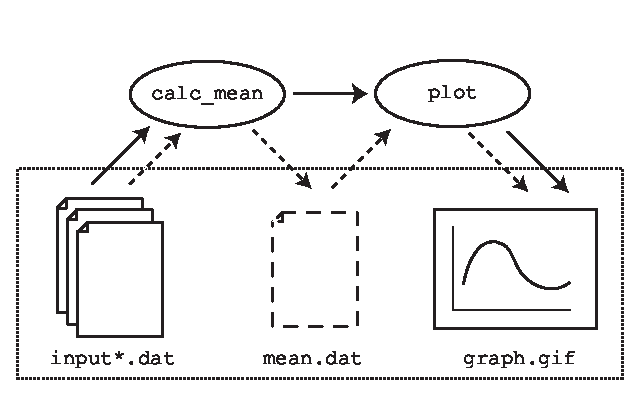
\includegraphics[height=8cm]{datapassing.eps}


\end{document}
